\chapter{Características de transferencia de corriente}

\section{Actividad de laboratorio}

\begin{figure}[H]
  \centering
  \begin{minipage}[b]{0.48\textwidth}
    \centering
    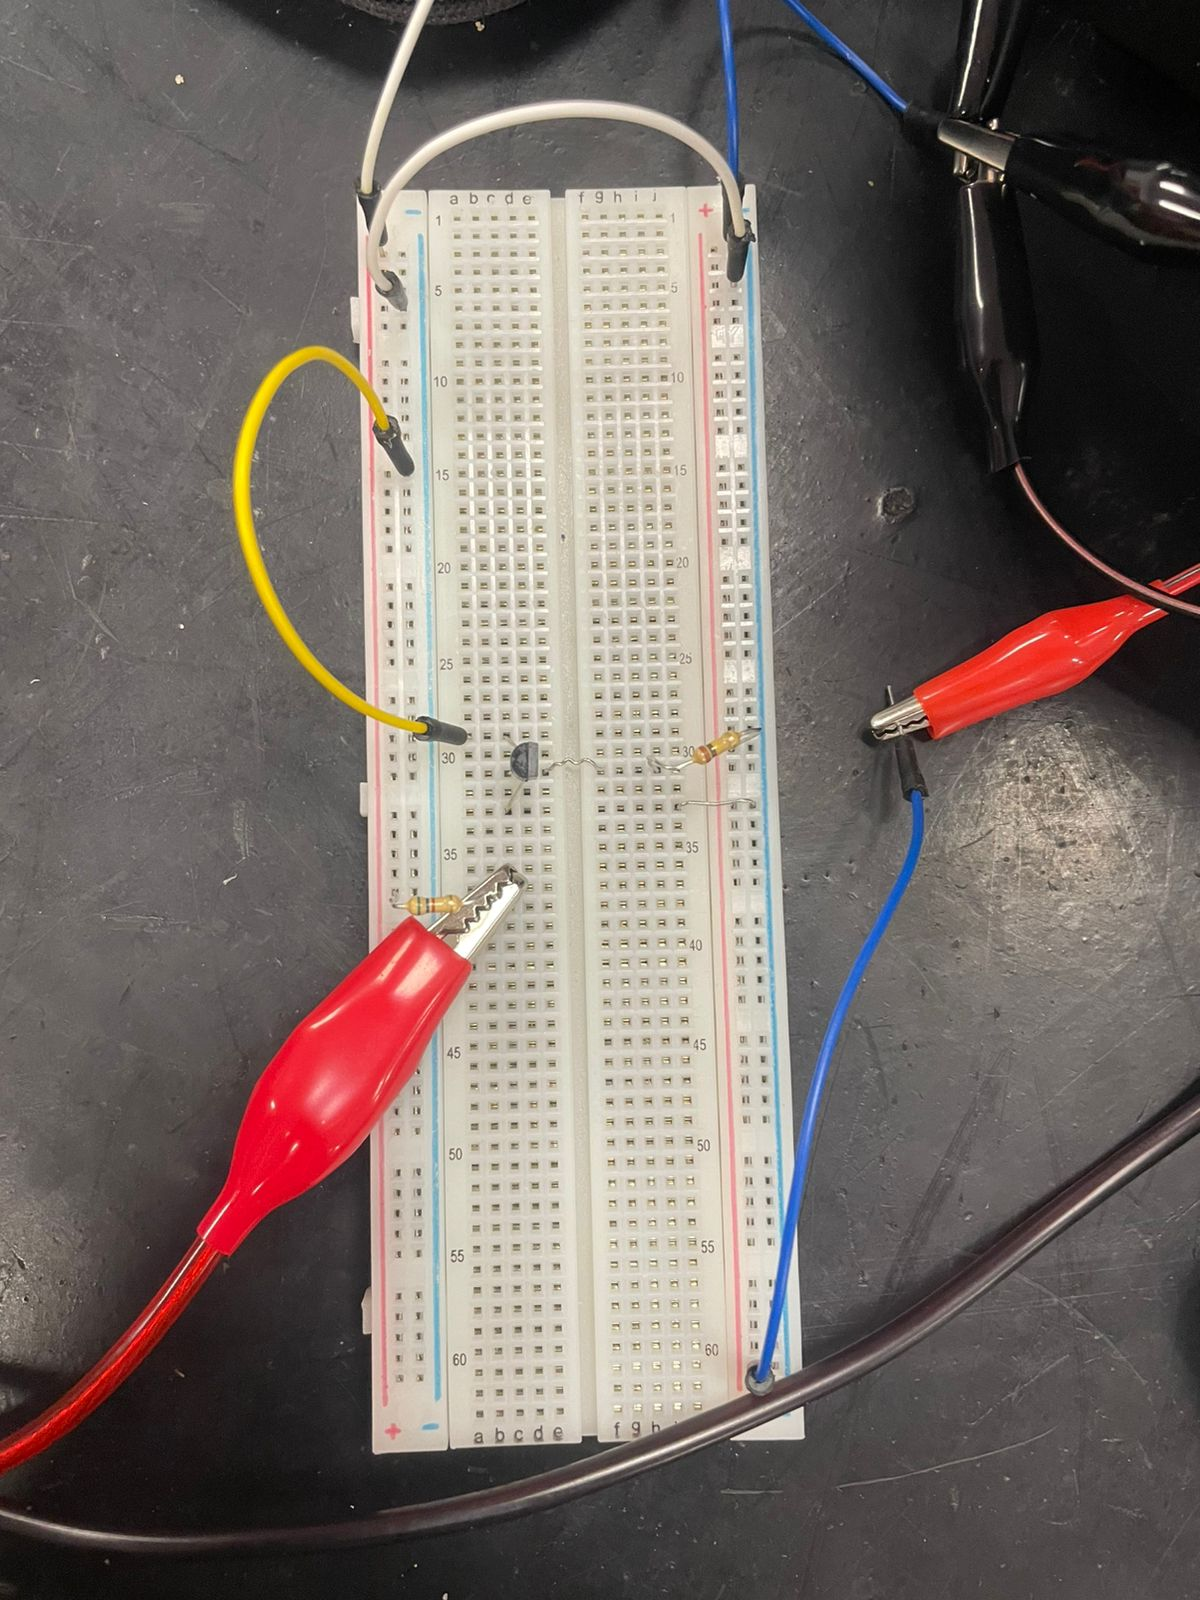
\includegraphics[width=\textwidth]{images/implementacion.jpg}
    \caption*{Implementacion del circuito}
  \end{minipage}
  \hfill
  \begin{minipage}[b]{0.48\textwidth}
    \centering
    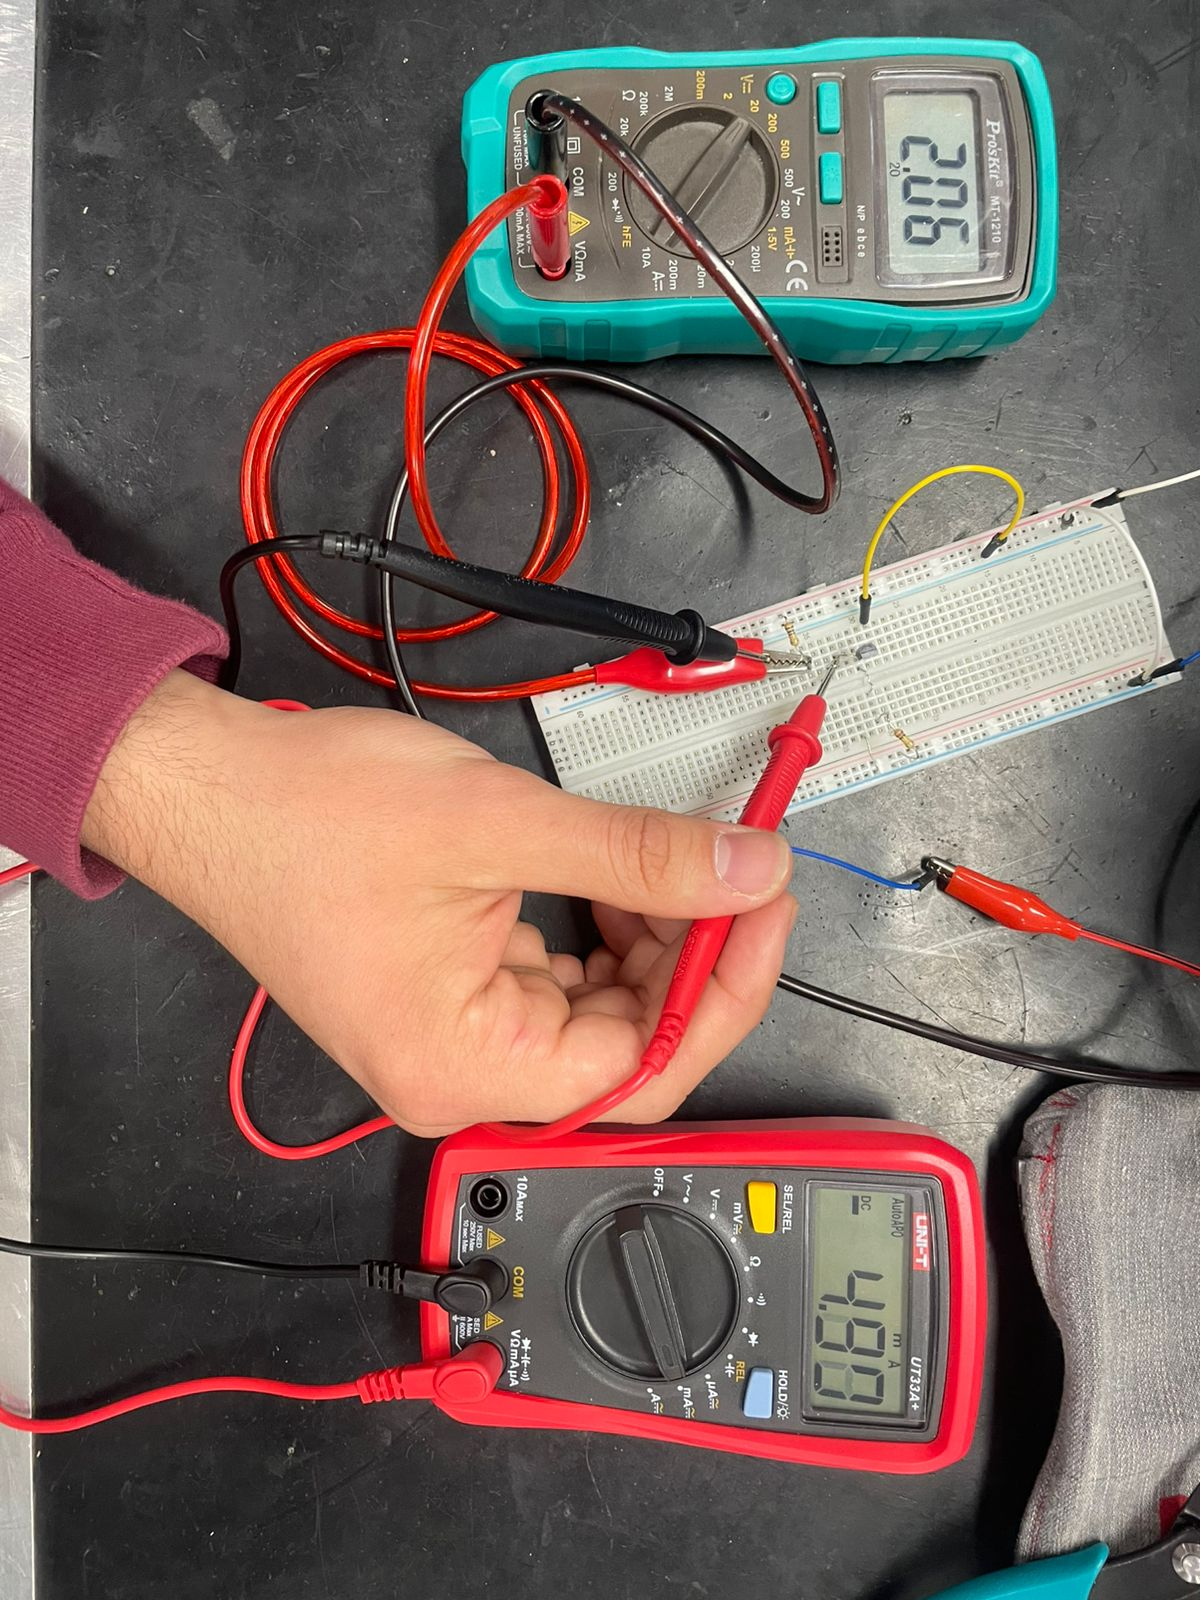
\includegraphics[width=\textwidth]{images/punto_3.jpg}
    \caption*{Realizacion de mediciones}
  \end{minipage}
\end{figure}

\begin{table}[H]
\centering
\begin{tabular}{|c|c|c|c|}
\hline
$I_B$ [$\mu$A] & $I_C$ (@$V_{CE(inicial)}$ = 2V) & $I_C$ (@$V_{CE(inicial)}$ = 5V) & $I_C$ (@$V_{CE(inicial)}$ = 8V) \\
\hline
5  & 900\,$\mu$A  & 920\,$\mu$A  & 933\,$\mu$A \\
7  & 1{,}46\,mA   & 1{,}5\,mA    & 1{,}52\,mA  \\
10 & 2{,}26\,mA   & 2{,}29\,mA   & 2{,}33\,mA  \\
20 & 5{,}00\,mA   & 5{,}15\,mA   & 5{,}18\,mA  \\
\hline
\end{tabular}
\caption{Tabla confeccionada.}
\end{table}

\section{Conclusión}

\newpage
